%!TEX root = TIWSNE_Mini_project_main.tex
\chapter{Introduction}
This report describes a mini project made as part of the masters degree programme in Information Technology at Aarhus University School of Engineering. The project was made in the Wireless Sensor Networks and Electronics course.

Wireless sensor networks consist of a number of battery powered sensor motes, whose operational lifetime is limited by how much energy they consume. In order to extend the lifetime, an effort is put into reducing the energy consumption of the nodes.    

\section{Goal}
The goal of this project is to asses image compression as a method of consuming less energy when transmitting an image from one sensor mote to another. Compressing the image prior to transmission will result in less data being transferred over the air, thereby reducing the energy consumed by the transceiver circuit in both motes. However a reduction in the total energy consumption depends on how much energy is consumed in the compression process.

\section{Description}
This project is concerned with the small sensor network shown in figure \ref{fig:blockDia}. 

\begin{figure}[H]
	\centering
	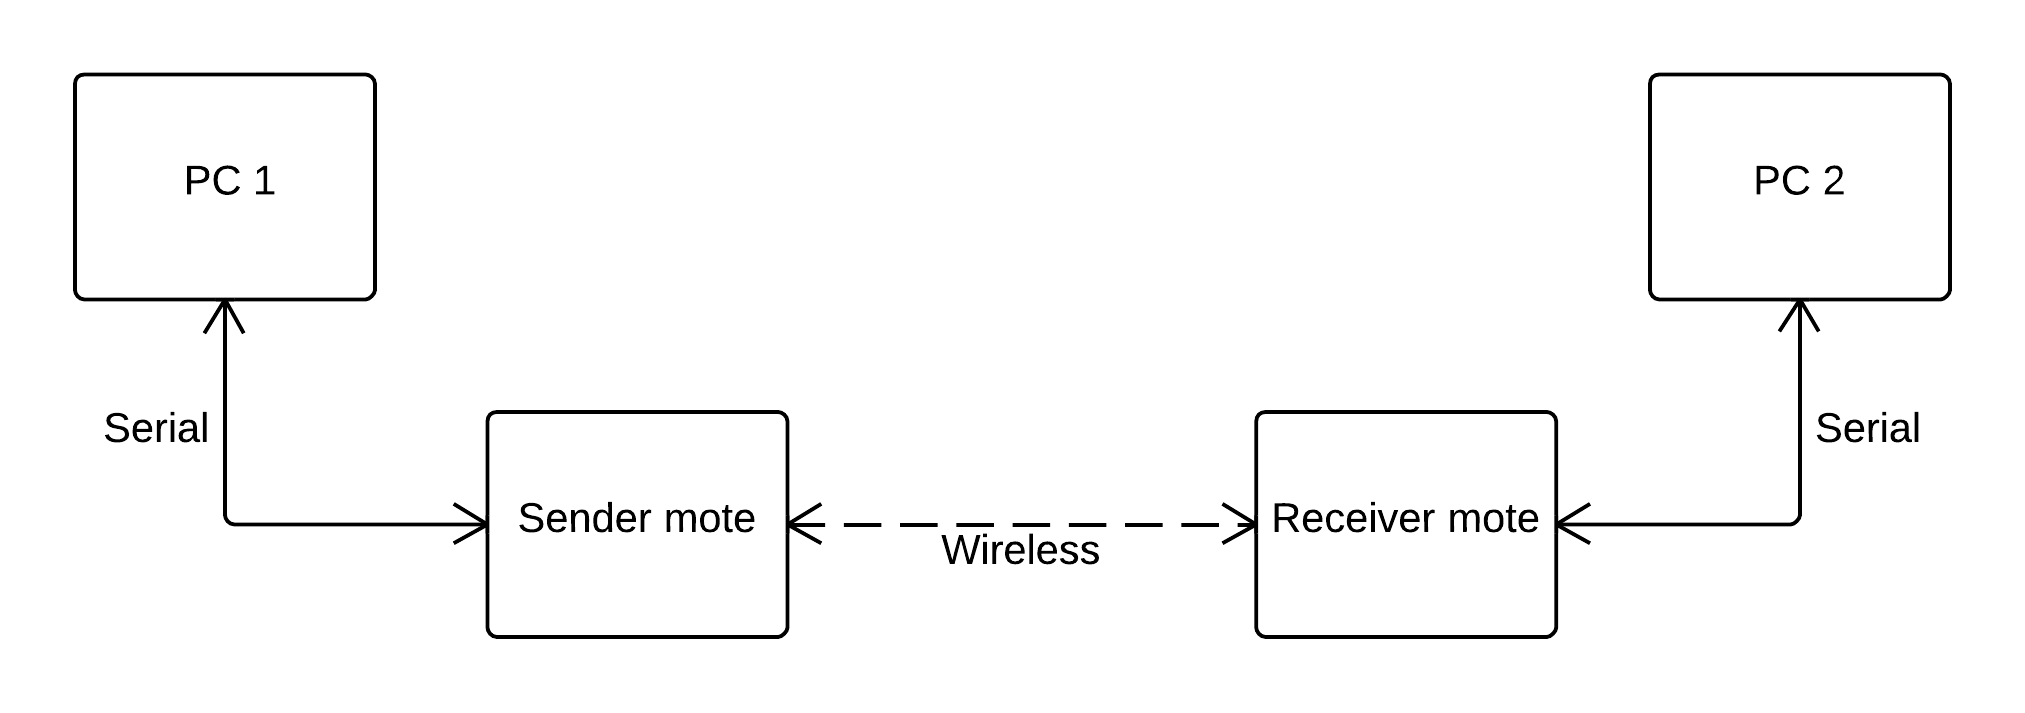
\includegraphics[width=\linewidth, scale = 0.7]{Figures/SimpleBlockDiagram}
	\caption{Block diagram with communication interfaces}
    \label{fig:blockDia}
\end{figure}

The network consists of two motes, a sender mote and a receiver mote, each connected to a PC via a serial connection. An image is loaded onto the sender mote from PC 1, and sent over the wireless channel to the receiver mote, from where it is transferred to PC 2. 
\\Energy consumption measurements of the communication between the motes is to be analysed with and without image compression, to determine its usefulness with regards to saving energy.

The following is to be implemented:
\begin{itemize}
\item A sensor mote application capable of sending and receiving both uncompressed and compressed images over both the wireless and serial channels.
\item A PC application capable of sending and receiving the image to and from the motes.
\end{itemize} 

The TelosB IEEE 802.15.4 wireless sensor module is used as hardware platform for the sensor motes.
 

